\section{\label{results}Results}

In Fig~\ref{fundamental_diagram_flow}, we show the fundamental diagram (density vs. flow) for different corridor's widths. In all the cases, the flow increases linearly with the density until $\rho=5$. When the density is grater than $\rho = 5$, we have two different scenarios:


\begin{itemize}
\item i) For narrow corridors (say $w < 10$) we can see that the flow reduces as the density increases. This resembles the traditional behavior of the fundamental diagram reported in the literature. 
\item ii) For wide corridors (say $w > 15$) we see that the flow increases with density. This contradicts the typical behavior of the fundamental diagram.   
\end{itemize}

We wonder what is the underlaying mechanism that produces these two distinctive behaviors. 

In order to satisfy the fundamental diagram reported in the literature, It is necessary that the flow at the maximum density ($\rho_{max} = 9$) be less than the flow at $\rho = 5$. That is:  $J(\rho = 9) < J(\rho = 5)$. From the flow definition in Ec.~\ref{ec-flow} we can derive

\begin{align*} 
v(\rho_{max}) &< \frac{5v_d}{\rho_{max}} \\
v(\rho_{max}) &< \frac{5}{9} v_d
\end{align*}



As our desired velocity is fixed $v_d = 1$~m/s, we conclude that the speed at the maximum density has to be bounded ($v(\rho_{max}) \lesssim 	0.5$) in order to satisfy the fundamental diagram reported in the literature.   

The above reasoning is consistent with the speed-density results shown in Fig.~\ref{fundamental_diagram_flow}. Notice that the speed values in $\rho_{max} = 9$ is higher than 0.5~m/s for $w=15$~m and $w=22$~m. Whereas the speed value for $\rho_{max}$ is lower than 0.5 for narrow corridors ($w<15$)

\begin{figure}[htbp!]
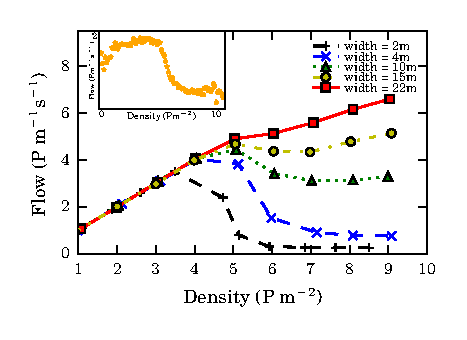
\includegraphics[width=\columnwidth]
{plots/flow-density_vd1_multiple_widths.eps}
\caption{\label{fundamental_diagram_flow} Flow as a function of the density for different widths. Initially, 
pedestrians were random distributed along the corridor. The measurements were taken in the middle
of the corridor once the system reached the stationary state. The length of the corridor 
was 28~m in all cases with periodic boundary conditions in the x direction.}
\end{figure}


\begin{figure}[htbp!]
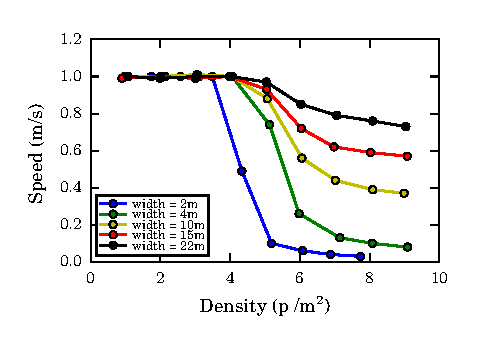
\includegraphics[width=\columnwidth]
{plots/speed-density_vd1_multiple_widths.eps}
\caption{\label{fundamental_diagram_speed} Speed as a function of the density for different widths. Initially, 
pedestrians were random distributed along the corridor. The measurements were taken in the middle
of the corridor once the system reached the stationary state. The length of the corridor 
was 28~m in all cases with periodic boundary conditions in the x direction.}
\end{figure}


\begin{comment}
\subsection{\label{evacuation}Evacuation time versus the desired velocity}

\begin{equation}
v^{-1}\sim \displaystyle\frac{\ln(\beta 
v_d/A)}{\beta v_d/A}\label{constrain2}
\end{equation}

\end{comment}
